% 第 1 章 方案总览
\chapter{方案总览}

\section{产品定位与价值主张}

\textbf{EdgeFlow 是什么}

EdgeFlow 是使用 Go 语言实现的云边端协同物联网平台，覆盖设备接入、边缘计算与云端统一管控场景，由云端与边缘两层软件栈构成：

\begin{itemize}
  \item \textbf{云端 CloudCore}：承担统一管控、REST API、审计台账与运行指标；
  \item \textbf{边缘 EdgeCore}：由 EdgeHub（云边通道）、Edged（容器自治）、DeviceTwin（设备影子）、EventBus（MQTT 数据面）、Mapper（设备接入）、MetaManager（SQLite 持久化）六个组件协同工作。
\end{itemize}

\textbf{解决什么问题}

\begin{enumerate}
  \item \textbf{设备接入与数据汇聚的标准化}：支持 MQTT、Modbus TCP 两类主流协议接入，遥测数据以统一 JSON 格式进入边缘 MQTT 数据面，屏蔽设备异构性（OPC-UA 接入\warn）；
  \item \textbf{边缘应用自治与弱网韧性}：以声明式调谐（默认 5s 调谐周期）持续将容器应用收敛到期望状态，支持多副本、健康自愈、CrashLoopBackOff 退避与镜像漂移检测，云边断连期间边缘采集与控制业务不中断；
  \item \textbf{管理与运维的可追溯性}：审计台账、keadm 升级回滚台账、设备操作台账三类台账覆盖 API 操作、系统变更与设备指令全链路，支撑审计与合规追溯；
  \item \textbf{生产级安全与轻量交付}：mTLS 云边通道、接入 Token、审计台账（文件 0600/目录 0700），keadm/Helm 一键部署，多架构镜像（linux/amd64 + arm64）。
\end{enumerate}

\textbf{价值主张}（结果性描述，不承诺 SLA 与收益数字）

\begin{itemize}
  \item \textbf{边缘自治}：应用期望状态由云端统一下发，边缘按声明持续调谐，减少现场人工干预；
  \item \textbf{弱网可用}：云边通道断开不中断边缘采集与设备控制，网络恢复后自动重连并周期补报最新状态；
  \item \textbf{全程可溯}：从 API 调用、系统升级到单条设备指令，均留有带时间戳与设备标识的台账记录；
  \item \textbf{快速落地}：keadm 初始化云端/接入边缘、Helm 部署云端、Docker 运行双端镜像，降低交付门槛。
\end{itemize}

\section{整体架构}

\begin{figure}[htbp]
  \centering
  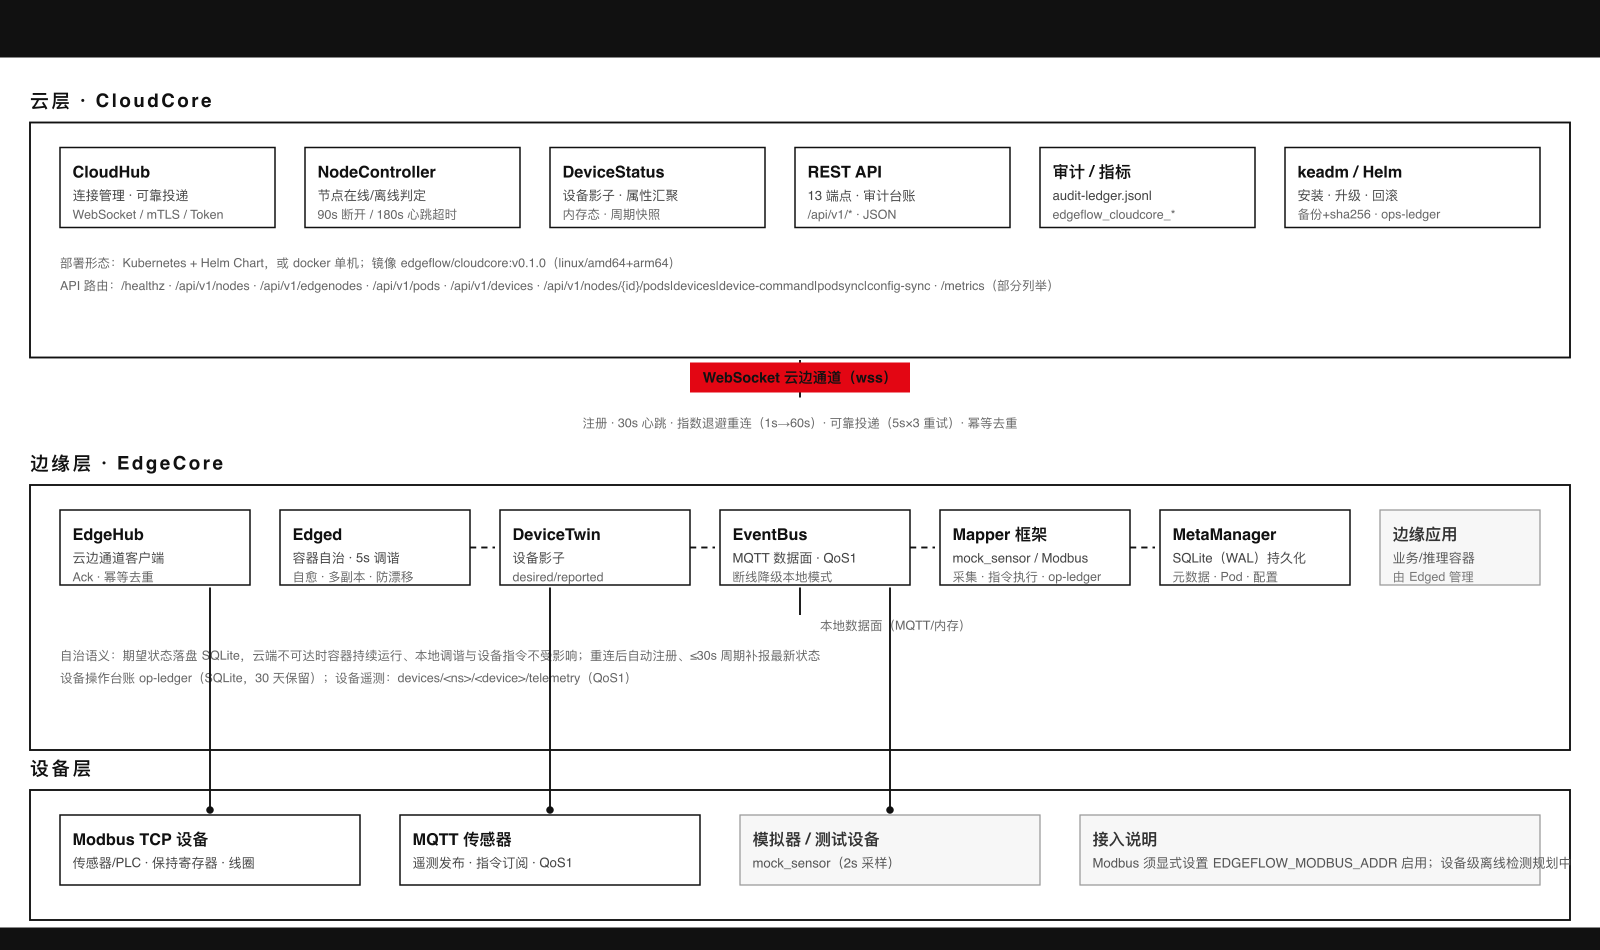
\includegraphics[width=0.94\textwidth]{../diagrams/arch-overview.png}
  \caption{EdgeFlow 整体方案架构}
  \label{fig:arch}
\end{figure}

EdgeFlow 采用“设备层—边缘层—云层”三层架构，文字版说明如下：

\textbf{设备层}：包括 Modbus TCP 设备、MQTT 传感器，以及用于演示与联调的模拟器 mock\_sensor（内存波动模拟遥测，2s 周期）。

\textbf{边缘层（EdgeCore）}，六个组件协作：

\begin{itemize}
  \item \textbf{Mapper}：设备接入与采集。Modbus 读保持寄存器（由 30s 上报循环驱动），采集结果写入 EventBus；
  \item \textbf{EventBus}：边缘 MQTT 数据面，承载遥测/指令主题，是 Mapper 与 DeviceTwin 之间的数据通道（QoS1）；
  \item \textbf{DeviceTwin}：设备影子，维护设备属性最新快照（内存态），并向云端周期上报；
  \item \textbf{MetaManager}：以 SQLite（WAL 模式）落盘节点元数据、Pod 期望状态与配置，提供边缘持久化；
  \item \textbf{Edged}：容器应用管理，按声明式调谐维护容器运行状态；
  \item \textbf{EdgeHub}：云边通信组件，通过 WebSocket 与云端 CloudHub 建立双向通道（支持退避重连）。
\end{itemize}

\textbf{云层（CloudCore）}，可部署于 Kubernetes（Helm Chart）或 Docker：

\begin{itemize}
  \item \textbf{CloudHub}：边缘节点连接管理；
  \item \textbf{NodeController}：节点状态维护；
  \item \textbf{DeviceStatus}：设备状态快照维护（内存态）；
  \item \textbf{REST API}：对外提供 14 个 HTTP 端点（11 个管理端点：设备、节点、命令、podsync/config-sync 等；另含 healthz 与 metrics）；
  \item \textbf{OCSP responder}：在线证书状态查询（POST /ocsp，RFC 6960；DER 编码请求/响应、免 Token——响应自带 CA 签名、16KiB 请求上限，状态码 200/400/429/500；per-IP 限流（默认 10 req/s、burst 20，超限 429，env 可调）+ 成功响应 Cache-Control: max-age=3600；与 CRL 同源 crl.json）；
  \item \textbf{审计与指标}：JSONL 审计台账 + 5 项运行指标。
\end{itemize}

\section{核心能力地图}

\textbf{表 1-1：四场景 × 特性组能力对照（v0.1.0 已实现 vs 规划中）}

{\small\setlength{\tabcolsep}{3pt}
\begin{tabular}{@{}p{1.3cm}p{1.3cm}p{6.4cm}p{6.0cm}@{}}
\toprule
场景 & 特性组 & v0.1.0 已实现 & 规划中/即将上线\\
\midrule
数据采集 & F21--F30 & MQTT/Modbus 设备接入；Mapper 周期采集（Modbus 30s 上报循环 / mock\_sensor 2s）；EventBus MQTT 数据面（QoS1）；设备影子与属性快照；设备命令下行（可靠投递 F05）；DeviceReport 周期上报（30s，可配） & OPC-UA 协议接入；设备级身份认证（节点接入 Token 认证已实现）\\
\addlinespace[3pt]
弱网自治 & F11--F20 & WebSocket 云边通道（gzip 协商式压缩）与退避重连；声明式调谐（5s）；多副本；健康自愈；CrashLoopBackOff；镜像漂移检测；MetaManager SQLite（WAL）持久化 & Flannel 网络；Protobuf 编码（gzip 通道压缩已实现）\\
\addlinespace[3pt]
模型管理 & F36--F39 & 镜像/配置下发通道（podsync/config-sync）；生产部署与升级回滚机制（升级分批灰度已工具化，见 4.2/4.4） & 模型仓库与版本管理；模型灰度发布（按节点/按比例）\\
\addlinespace[3pt]
模型应用 & F11--F19 & 容器应用部署与自治：多副本、健康自愈、CrashLoopBackOff、镜像漂移检测 & 模型灰度发布；调度/超卖\\
\bottomrule
\end{tabular}}

\begin{quote}
注：特性编号沿用产品特性基线；同一编号区间在不同场景视图下以该场景语义为准。
\end{quote}

\section{版本与发布信息}

\textbf{版本信息}：EdgeFlow v0.1.0，发布日期 2026-08-14。

\textbf{制品清单（表 1-2）}

\begin{tabularx}{\textwidth}{p{2.2cm}X}
\toprule
类别 & 制品\\
\midrule
容器镜像 & edgeflow/cloudcore:v0.1.0、edgeflow/edgecore:v0.1.0（linux/amd64 + arm64 多架构）\\
部署工具 & keadm（init/join/cert(rotate|revoke)/upgrade/rollback/ops-ledger/batch/reset/version，共 9 个子命令）、Helm Chart（云端）、Docker（双端运行）\\
接口能力 & REST API 14 端点（11 管理 + healthz + metrics + /ocsp）；运行指标 5 项；OpenAPI v3 schema（\seqsplit{\texttt{docs/openapi/edgeflow-openapi.yaml}}，\seqsplit{\texttt{hack/gen-openapi.sh}} 自动生成，勿手编）；API 兼容性契约测试（\seqsplit{\texttt{tests/contract}}，14 端点）\\
\bottomrule
\end{tabularx}

\textbf{v0.1.0 功能范围（已实现）}：WebSocket 云边通道（gzip 协商式压缩：Register 协商、v1.0 兼容、\seqsplit{\texttt{config/cloudcore.json}} 中 \texttt{compress:false} 可关）；边缘容器自治（声明式调谐 5s、多副本、健康自愈、CrashLoopBackOff、镜像漂移检测）；设备管理（MQTT/Modbus 接入、设备影子、设备命令）；节点接入认证（\env{EDGEFLOW\_EDGECORE\_TOKEN}，云端常数时间校验、空值向后兼容）；证书生命周期管理（keadm cert rotate/revoke，CRL 离线 + OCSP 在线应答）；配置管理（\seqsplit{\texttt{config/edgecore.json}}，环境变量 > 配置文件 > 默认值，SIGHUP + 60s 热重载）；升级回滚与灰度（\seqsplit{\texttt{keadm batch --op=upgrade}} + \texttt{--batch-size}/\texttt{--pause-between}）；生产加固（mTLS/Token/审计台账/keadm/Helm/多架构镜像）；发布流程级镜像安全扫描（构建期 Trivy，基线 0 漏洞）；接口工程（OpenAPI v3 schema + 契约测试）。

\textbf{\warn}：模型仓库与版本管理、模型灰度发布（升级分批灰度已工具化）、完整 RBAC（当前为单 Token 鉴权）、设备级身份认证（节点接入认证已实现）、调度/超卖、Flannel 网络、OPC-UA 接入、Protobuf 编码（gzip 通道压缩已实现）、产品内置镜像安全扫描（发布流程构建期 Trivy 扫描已建立，基线 0 漏洞）。
